%=============================================================================
\section{Experiments: Synthetic Diagnostics and Real-LLM Evaluation}
\label{sec:experiments}

We test every theoretical prediction in two stages: controlled Monte Carlo
verification of our closed-form bounds (including fixes for historical scaling
and contamination artifacts detailed in Appendix~\ref{app:experiments}), followed
by held-out validation on two public human-annotated LLM benchmarks using zero
human labels during unsupervised aggregation.

\begin{figure}[t]
  \centering
  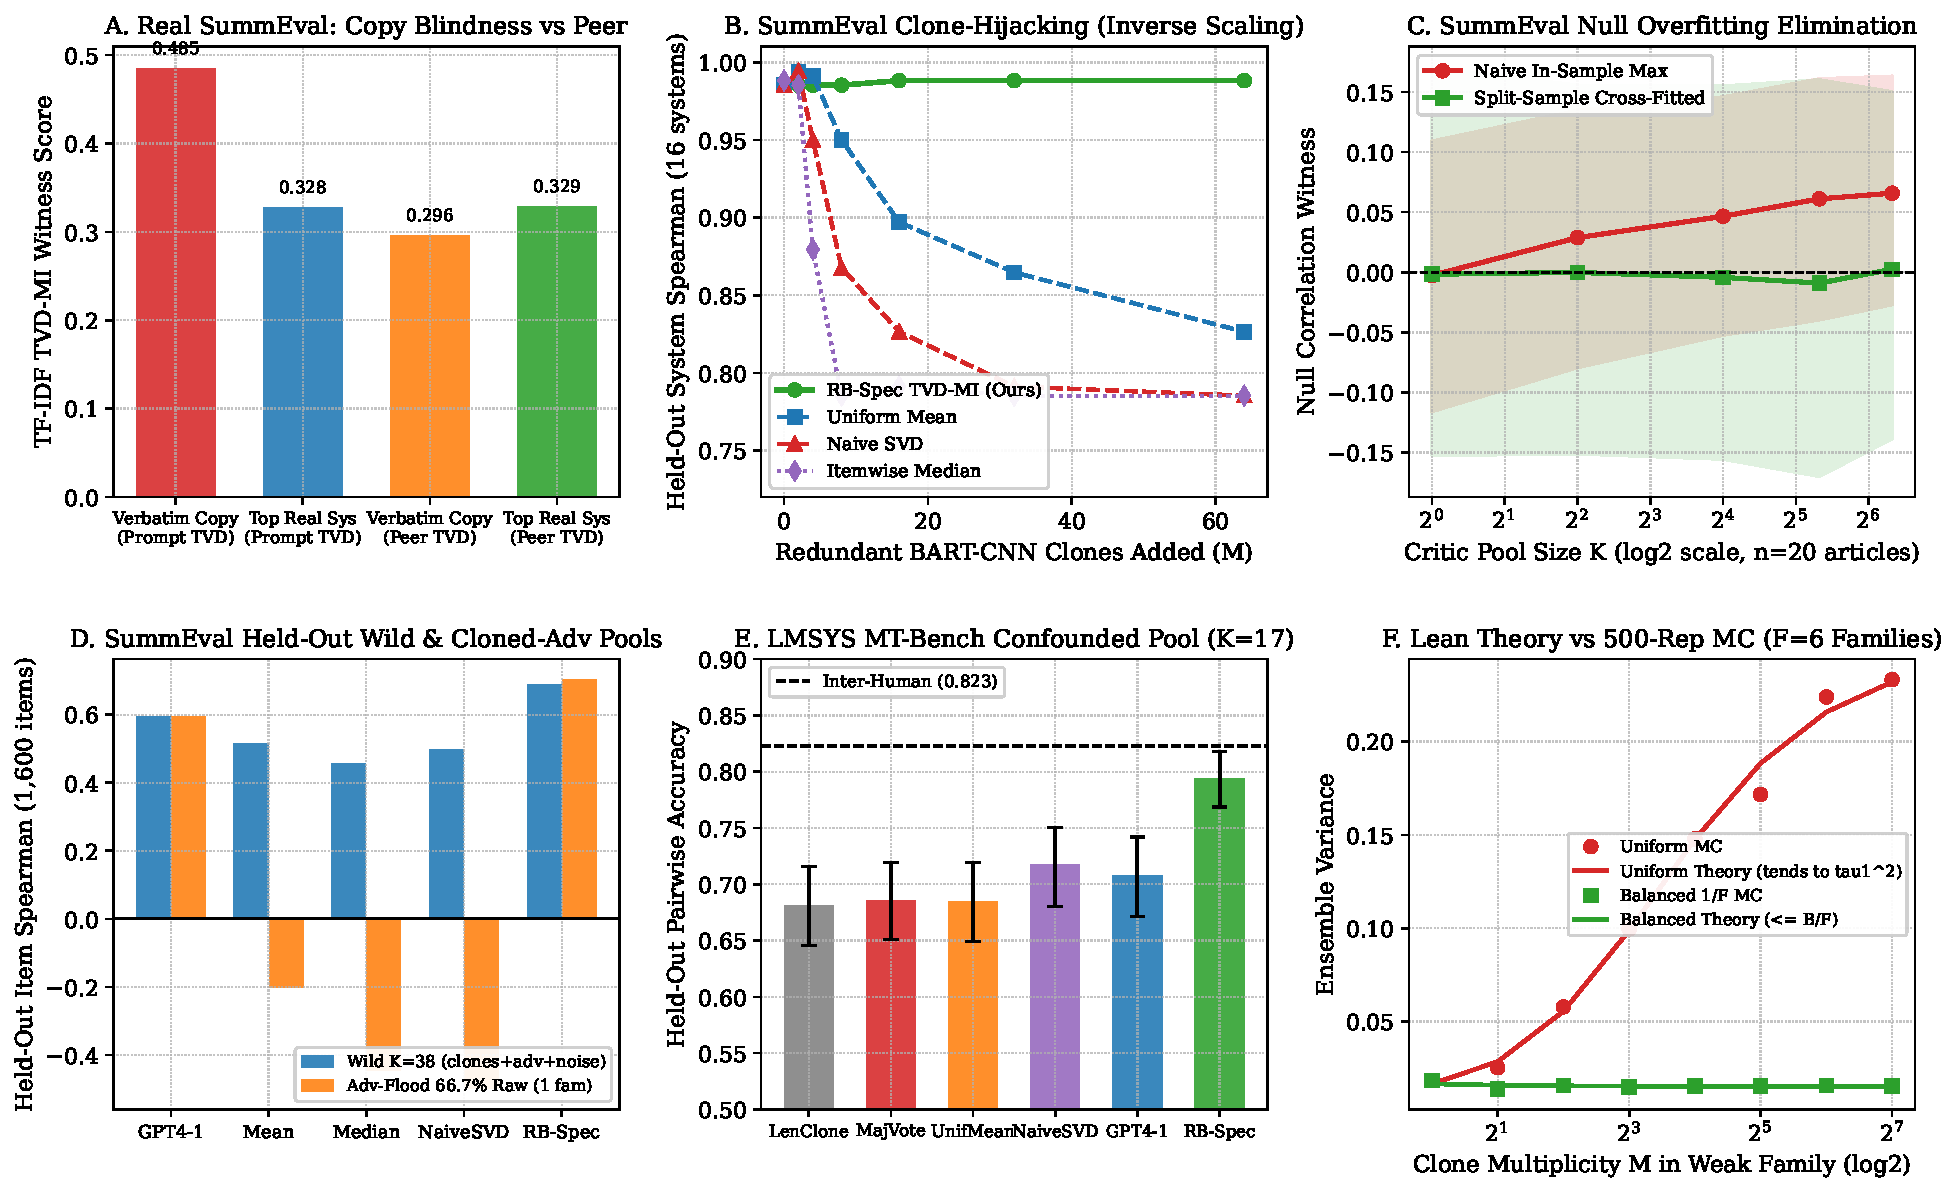
\includegraphics[width=\textwidth]{figures/exp13_real_llm_and_theory_6panel.pdf}
  \caption{\textbf{Real-LLM and theoretical verification (Experiment~13, 5-fold cluster-held-out evaluation).}
  \textbf{(A)} On \textsc{SummEval}, verbatim prompt copying ($0.485$) scores above the strongest real summarizer ($0.328$) under prompt--response TVD-MI, whereas peer contrast restores separation ($0.329$ vs.\ $0.296$).
  \textbf{(B)} Adding $M \in \{0,\dots,64\}$ prompt clones of \texttt{BART-CNN} causes uniform averaging ($0.985 \to 0.826$), itemwise medians ($0.988 \to 0.785$), and naive SVD ($0.985 \to 0.785$) to degrade, while \texttt{RB-Spec TVD-MI} remains flat ($0.988$).
  \textbf{(C)} On \textsc{SummEval} null permutations ($n=20$ articles), naive in-sample maximization inflates to $+0.065$, while split-sample selection stays unbiased ($+0.001$, $p=0.992$).
  \textbf{(D)} Under wild ($K=38$) and cloned-adversarial ($66.7\%$ raw adversaries in 1~family) pools, \texttt{RB-Spec TVD-MI} achieves $+0.689$ and $+0.703$ item Spearman while mean, median, and naive SVD collapse to $[-0.500, -0.201]$ under cloned adversaries.
  \textbf{(E)} On \textsc{MT-Bench} ($K=17$ confounded pool, $2,575$ human pairs), \texttt{RB-Spec} reaches pairwise accuracy $0.795$ near the inter-human ceiling ($0.823$).
  \textbf{(F)} Five-hundred-rep Monte Carlo simulations match Theorem~\ref{thm:balanced-1F} and Proposition~\ref{prop:clone-hijacking}.}
  \label{fig:exp13-overview}
\end{figure}

% Provenance: experiments/13_real_llm_validation_hierarchical_rb_spectral_theory_and_lean_start_21Nov2026/results/summary_metrics.json, summeval_heldout_regimes.csv, mtbench_pairwise.csv
\subsection{Real-LLM Benchmarks and Unsupervised Evaluation Protocol}

\textbf{\textsc{SummEval} \citep{fabbri2021summeval}.} We evaluate $1,600$ summaries
across $100$ articles and $16$ summarization systems against the three-expert mean
across four quality dimensions (human overall mean $4.131$; leave-one-expert-out
ceiling: item Spearman $0.758\,[0.729, 0.782]$, system Spearman $0.966$,
$\mathrm{ICC(A,1)} = 0.806$). The reference-free judge pool combines $4$ single-sample
GPT-4 G-Eval critics (\citealp{liu2023geval}; valid parses $31{,}809/32{,}000$ to
$32{,}000/32{,}000$), $4$ diverse sequence-to-sequence models
(\texttt{BARTScore}, \texttt{BART-para}, \texttt{BART-CNN}, \texttt{PRISM}),
$70$ paraphrased \texttt{BART-CNN} prompt variants, and candidate word length.
All unsupervised ensemble weights are fitted strictly within each training fold
via 5-fold article-disjoint cross-validation, using raw training GPT-4 Likert
means solely to anchor the $[1,5]$ output scale without accessing human scores.

\textbf{\textsc{LMSYS MT-Bench} \citep{zheng2023judging}.} Over all $2,575$
decisive human pairwise judgments spanning $80$ multi-turn questions and $6$ chat
models (inter-human agreement $0.823$ across $779$ repeated pairs), we construct a
$K=17$ confounded pairwise pool pairing the released GPT-4 pairwise judge, prompt-specificity
TF-IDF similarity, lexical diversity, $11$ verbosity-length clones, and $3$
sign-flipped adversarial critics via 5-fold question-disjoint cross-validation.
Uncertainty is reported via $2,000$ article- or question-cluster bootstrap draws
($x\,[l, u]$) and paired Wilcoxon tests across independent clusters.

\begin{table}[t]
\centering
\caption{\textbf{Held-out 5-fold real-LLM evaluation} on \textsc{SummEval}
($100$ articles, $1,600$ items) and \textsc{MT-Bench} ($80$ questions, $2,575$
decisive human pairs); $95\%$ cluster-bootstrap intervals.}
\label{tab:real-llm-main}
\resizebox{\textwidth}{!}{%
\begin{tabular}{@{}lcccc@{}}
\toprule
Method & \textsc{SummEval} Wild ($K=38$) & \textsc{SummEval} Adv-Flood ($67\%$ raw) & \textsc{SummEval} Sys Sp.\ (Adv) & \textsc{MT-Bench} Pair Acc. \\
\midrule
Single GPT-4 & $0.596\,[0.557, 0.634]$ & $0.596\,[0.556, 0.633]$ & $0.965\,[0.900, 0.976]$ & $0.708\,[0.671, 0.742]$ \\
Uniform Mean & $0.515\,[0.466, 0.561]$ & $-0.201\,[-0.269, -0.131]$ & $-0.265\,[-0.468, -0.094]$ & $0.685\,[0.649, 0.720]$ \\
Itemwise Median & $0.457\,[0.398, 0.513]$ & $-0.446\,[-0.505, -0.387]$ & $-0.785\,[-0.853, -0.665]$ & $0.686\,[0.651, 0.720]^\dagger$ \\
Naive Rank-1 SVD & $0.497\,[0.446, 0.547]$ & $-0.500\,[-0.550, -0.450]$ & $-0.806\,[-0.891, -0.673]$ & $0.718\,[0.681, 0.751]$ \\
\textbf{\texttt{RB-Spec TVD-MI}} & $\mathbf{0.689\,[0.659, 0.718]}$ & $\mathbf{0.703\,[0.673, 0.732]}$ & $\mathbf{0.974\,[0.903, 0.979]}$ & $\mathbf{0.795\,[0.769, 0.820]}$ \\
\bottomrule
\end{tabular}}
\vspace{2pt}
{\footnotesize $^\dagger$Majority Vote on pairwise decisions. \texttt{RB-Spec} improves over Uniform Mean with Wilcoxon $p=1.21\times 10^{-9}$ (Wild), $p=4.40\times 10^{-18}$ (Adv-Flood), and $p=3.87\times 10^{-10}$ (\textsc{MT-Bench}).}
\end{table}

\subsection{Headline Findings and Absolute Agreement Caveat}

As shown in Figure~\ref{fig:exp13-overview} and Table~\ref{tab:real-llm-main}:
(1)~\textbf{Pairwise residual correlation saturation} occurs sharply within model
families ($\rho = 0.769$ across $20$ stochastic GPT-4 calls; $\rho = 1.000$ across
$70$ \texttt{BART-CNN} prompts) compared to distinct families ($\rho = 0.558$);
(2)~\textbf{Clone hijacking is reversible unsupervised}: adding $64$ redundant
clones degrades Uniform Mean by $-0.159$ system Spearman and Naive SVD by $-0.200$
(across $200$ repeated $50/50$ splits, \texttt{RB-Spec} obtains $0.970\,[0.935, 0.991]$
vs.\ Uniform Mean $0.806\,[0.712, 0.874]$, $p=1.43\times 10^{-34}$); and
(3)~\textbf{Raw uncalibrated level bias persists without human anchors}: while
\texttt{RB-Spec TVD-MI} attains strong rank and linear tracking ($\mathrm{ICC(C,1)}=0.688$,
item Pearson $0.726\,[0.702, 0.749]$ on Wild $K=38$), the pooled uncalibrated G-Eval
anchor mean ($3.019$) sits below expert severity ($4.131$), yielding mean bias
$-1.111\,[-1.168, -1.052]$ and $\mathrm{ICC(A,1)}=0.351$.
